\documentclass[xetex, xcolor=dvipsnames]{beamer}
\usepackage{animate}
\usepackage{style}
\usepackage{symbols}
\usepackage{comment}
\mode<presentation>

% \institute{Дальневосточный Федеральный Университет}
\title{
	Численный анализ диффузионных моделей распространения вирусов 
}
\subtitle{}
\author{
	Максимов П.А. \\ \vspace{10pt}
	Научный руководитель: \\ к.ф.-м.н. Бризицкий Р.В., д.ф.-м.н. Алексеев Г.В.
}
\date{Владивосток, 2022}

\begin{document}
	
	\begin{noheadline}
		\frame {
			\fefuheader
			\titlepage
		}
	\end{noheadline}

	\frame {

		\frametitle{Основные положения}

		Исследуются краевые и экстремальные задачи для нелинейных уравнений реакции-диффузии-конвекции.

		Коэффициенты в уравнениях и граничных условиях рассматриваемых моделей нелинейно зависят от концентрации вещества, а также зависят от пространственной переменной.

		\textbf{Краевые задачи}
		\begin{enumerate}
			\item Глобальная разрешимость и локальная (или нелокальная) единственность решений;
			% \item Принцип максимума и минимума для концентрации вещества.
		\end{enumerate}

		\textbf{Задачи управления}
		\begin{enumerate}
			\item Разрешимость задач управления в общем виде;
			\item Вывод систем оптимальности;
			\item Оценки локальной устойчивости оптимальных решений.
		\end{enumerate}

	}

	\frame {

		\frametitle{План доклада}

		\begin{enumerate}
			\item Постановка и разрешимость краевых задач для нелинейного уравнения реакции-диффузии-конвекции;
			% \item Принцип максимума и минимума для линейного уравнения реакции-диффузии-конвекции при смешанных краевых условиях;
			% \item Принцип максимума для нелинейного уравнения реакции-диффузии-конвекции;
			\item Задача мультипликативного управления и нелинейные модели;
			\item Оценки локальной устойчивости;
			\item Численный анализ для диффузионных моделей распространения вирусов.
		\end{enumerate}
	}

	\frame {

		\frametitle{Краевая задача}

		В ограниченной области \( \Omega \subset \R^{3} \) с границей $\Gamma$ рассматривается следующая краевая задача:

		\begin{equation}
			\label{4a}
			\begin{split}
				- \div{(\lambda(\mathbf{x}) \grad{\vp})} 
				+ \mathbf{u} \cdot \grad{\vp}
				+ k (\vp, \mathbf{x}) \vp 
				= f ~ \text{ в } \Omega, \\ 
				\vp = \psi ~ \text{ на } \Gamma 
			\end{split}
		\end{equation}

		Здесь:
		\begin{itemize}
			\item \( \vp \) -- концентрация вещества,
			\item \( \mathbf{u} \) -- заданный вектор скорости,
			\item \( \lambda = \lambda(\mathbf{x}) > 0 \) -- коэффициент диффузии,
			\item \( f \) -- объемная плотность внешних источников,
			\item \( k = k(\vp, \mathbf{x}) \) -- коэффициент реакции,
		\end{itemize}

	}

	\frame {

		\frametitle{Функциональные пространства и условия}
		
		Пространство для вектора скорости \( \mathbf{u} \):
		\[ 
			Z = \braces{ 
				\mathbf{u} \in L^4 (\Omega)^3: 
				\div{\mathbf{u}} = 0
			},
		\] 
		Пространство для коэффициента диффузии \( \lambda \):
		\[ 
			H^{s}_{\lambda_0} (\Omega) = \braces{ 
				\lambda \in H^{s} (\Omega): \lambda \ge \lambda_0 > 0 \text{ в } \Omega 
			}, s > 3/2, 
		\] 

		\begin{enumerate}%[i]

			\item 
				\label{iareac1}
				\( \Omega \in \R^3 \) -- ограниченная область с границей $\Gamma \in C^{0, 1}$,

			\item 
				\label{iareac2}
				\( \lambda \in H^{s}_{\lambda_0}(\Omega), ~ s > 3/2, ~ \mathbf{u} \in Z, ~ f \in L^2(\Omega), ~ \psi \in H^{1/2}(\Gamma). \)

		\end{enumerate}
	}

	\frame {
		
		\frametitle{Коэффициент реакции}

		\begin{enumerate}%[i]

			\setcounter{enumi}{2}
			\item 
				\label{iareac3}
				\( k(v, \cdot) \in L^{p}_{+}(\Omega), ~ p \ge 5/3, ~ \forall v \in H^{1}(\Omega) \), и на шаре
				\[ B_r = \braces{ v \in H^1(\Omega) : ~ \norm{v}_{1, \Omega} \le r } \]
				справедливо неравенство

				\vspace*{-10pt}
				\[ \norm{k(v_1, \cdot) - k(v_2, \cdot)}_{L^{p}(\Omega)} \le L_1 \norm{v_1 - v_2}_{L^4(\Omega)} ~ \forall v_1, v_2 \in B_r. \]
				Здесь $L_1$ -- константа, зависящая от $r$, но не зависящая от \( v_1, v_2 \in B_r \).

		\end{enumerate}
	}

	\frame {
		
		\frametitle{Условия на коэффициент реакции}

		\begin{enumerate}%[i]
			\setcounter{enumi}{3}

			\item \label{iareac4}
				Пусть \( \Omega_1 \subset \Omega \) такая подобласть области $\Omega$, что \( \overline{\Omega}_1 \subset \Omega \). \( k \pares{\vp,\cdot} \vp \) -- монотонна в \( \Omega_2 = \Omega \setminus \overline{\Omega}_1 \):
				\[ \pares{ k (\vp_1, \cdot) \vp_1 - k (\vp_2, \cdot) \vp_2, \vp_1 - \vp_2} \ge 0 ~ \forall \vp_1, \vp_2 \in H^1 (\Omega), \]

		\end{enumerate}
		и ограниченной в следующем смысле:
		\begin{enumerate}%[i]
			\setcounter{enumi}{4}

			\item \label{iareac5}
				\( \norm{ k (\vp, \cdot) }_{L^p (\Omega_2)} \le A_1 \norm{\vp}_{1,\Omega}^r + B_1 ~ \forall \vp \in H^1 (\Omega), ~ p \ge 5/3, r \ge 0 \),

		\end{enumerate}
		а в \( \Omega_1 \) справедливо неравенство:
		\[ \norm{k(\vp, \cdot)}_{L^p(\Omega_1)} \le C_1 \forall \vp \in H^1(\Omega). \]

	}

	\frame {

		\frametitle{Разрешимость краевой задачи}

		Пример:
		\vspace*{-8pt}
		\[ k = \frac{1}{1 + \vp^2} \text{ в } \Omega_1 \text{ и } k = \vp^2 \text{ в } Q \subset \Omega_2, ~ k = k_0(\mathbf{x}) \subset L^{5/3}_{+}\pares{\Omega_2 \setminus \overline{Q}} \text{ в } \Omega_2 \setminus \overline{Q}. \]

		\begin{block}{Теорема 1.}
			\label{thref11}
			При выполнении условий (\ref{iareac1})--(\ref{iareac5}) существует слабое решение $\vp \in H^1 (\Omega)$ задачи 1, для которого справедлива оценка
			\begin{equation}
				\label{est_phi}
				\begin{split}
					\norm{\vp}_{1,\Omega} \le &M_\vp \equiv 
						C_* \left({\norm{f}_{\Omega} + 
							C_{\Gamma} \pares{C_0 \norm{\lambda}_{s, \Omega} + \gamma_1 \norm{\mathbf{u}}_{L^4(\Omega)^3} + \gamma_p C_1} \norm{\psi}_{1/2, \Gamma} 
						}\right. + \\
						& \left. 
							+ C_{*} \gamma_p C_{\Gamma} 
							\pares{C_{\Gamma}^r A_1 \norm{\psi}_{1/2, \Gamma}^r + B_1} \norm{\psi}_{1/2, \Gamma} 
						\right) + C_{\Gamma} \norm{\psi}_{1/2,\Gamma}.
				\end{split}
			\end{equation}

			Если к тому же, выполняется условие \( \gamma_p L M_{\vp} < \lambda_{*} \), то слабое решение задачи 1 единственно.

		\end{block}
	}

	\begin{comment}

		\frame {

			\frametitle{Принцип максимума и минимума}

			Дополнительные условия на исходные данные:

			\begin{enumerate}
				\setcounter{enumi}{5}
				\item \label{iareac6}
					\( \psi_{\min} \le \psi \le \psi_{\max} \) п.в. на $\Gamma$, \( f_{\min} \le f \le f_{\max} \) п.в. в \( \Omega_2 \), $f = 0$ п.в. в $\Omega_1$ (либо \( \Omega_1 = \emptyset \) )

				\item \label{iareac7}
					\( k(\vp, \mathbf{x}) = a(\mathbf{x}) k_1(\vp) \), где \( k_1(\cdot) : \R \to \R_{+} \) непрерывная функция, \( 0 < a_{\min} \le a(\mathbf{x}) \le a_{\max} < \infty \) п.в. в $\Omega$, причем функциональные уравнения
					\[ k_1(s) s = f_{\max}/a_{\min} ~ \text{ и } ~ k_1(s) s = f_{\min}/a_{\max} \]
					имеют хотя бы одно решение.

			\end{enumerate}
		}

		\frame {

			\begin{block}{Лемма 1.}
				\label{lemm11}
				При выполнении условий (\ref{iareac1})--(\ref{iareac7}) для решения \( \vp \in H^1(\Omega) \) задачи 1 справедлив следующий принцип максимума и минимума:
				\[ m \le \vp \le M \text{ п.в. в } \Omega, \]
				\[ M = \max \braces{ \psi_{\max}, M_1 }, ~ m = \min \braces{ \psi_{\min}, m_1 }. \]

				Здесь $M_1$ -- минимальный корень уравнения
				\[ k_1(s) s = f_{\max}/a_{\min}, \]
				а $m_1$ -- максимальный корень уравнения
				\[ k_1(s) s = f_{\min}/a_{\max}. \]

			\end{block}

			Пример: 
			\[
				k(\vp) = \vp^2, \quad k(\vp) \vp = \vp^3 = f_{\max}, \quad M_1 =f_{\max}^{1/3}.
			\]
		}

	\end{comment}

		
	\frame {

		\frametitle{Краевая задача №2}

		В ограниченной области \( \Omega \subset \R^{3} \) с границей $\Gamma$, состоящей из двух частей \( \Gamma_D \) и \( \Gamma_N \) рассматривается следующая краевая задача:

		\begin{equation}
			\label{4a}
			\begin{split}
				- \div{(\lambda(\mathbf{x}) \grad{\vp})} 
				+ \mathbf{u} \cdot \grad{\vp}
				+ k (\vp, \mathbf{x}) \vp 
				= f ~ \text{ в } \Omega, \\ 
				\vp = \psi ~ \text{ на } \Gamma_D, \\
				\lambda(\mathbf{x}) 
					\left( 
						\partial \vp / \partial n + \alpha(\vp, \mathbf{x})\vp 
					\right)
				=\chi \text{ на } \Gamma_N. 
			\end{split}
		\end{equation}

		Здесь:
		\begin{itemize}
			\item \( \alpha = \alpha(\vp, \mathbf{x}) \) -- коэффициент массообмена,
			\item \( \chi \) -- объемная плотность граничных источников.
		\end{itemize}
	}
	%Упрощенная система оптимальности (3 phi ^2 tau, проверить оценку 7)

		\frame {
			\frametitle{Функциональные пространства и условия}

			\[ 
				\cT = \braces{
					h \in H^1(\Omega): h \ont_{\Gamma_D} = 0
				},
			\]
			\[ 
				Z = \braces{ 
					\mathbf{u} \in L^4 (\Omega)^3: 
					\div{\mathbf{u}} = 0
					\text{ в } \Omega, 
					~ \mathbf{v \cdot n}\ont_{\Gamma_N} = 0 
				},
			\] 
			\[ 
				H^{s}_{\lambda_0} (\Omega) = \braces{ 
					\lambda \in H^{s} (\Omega): \lambda \ge \lambda_0 > 0 \text{ в } \Omega 
				}, s > 3/2.
			\] 
			
			\begin{enumerate}%[i]

				\item 
					\label{icreac1}
					\( \Omega \in \R^3 \) -- ограниченная область с границей $\Gamma \in C^{0, 1}$, состоящей из замыканий двух непересекающихся открытых участков \( \Gamma_D \) и \( \Gamma_N \)

					\[ \Gamma = \overline{\Gamma}_D \cup \overline{\Gamma}_N, ~ \Gamma_D \cap \Gamma_N = \emptyset, ~ \meas{\Gamma_D} > 0; \]
				\item 
					\label{icreac2}
					\( \lambda \in H^{s}_{\lambda_0}(\Omega), ~ s > 3/2, ~ \mathbf{u} \in Z, ~ f \in L^2(\Omega), ~ \psi \in H^{1/2}(\Gamma_D), ~ \chi \in L^2(\Gamma_N). \)

			\end{enumerate}
		}
		
	\begin{comment}

		\frame {
			
			\frametitle{Коэффициенты реакции и массообмена}

			\begin{enumerate}%[i]

				\setcounter{enumi}{2}
				\item 
					\label{icreac3}
					\( k(v, \cdot) \in L^{p}_{+}(\Omega), ~ p \ge 3/2, ~ \forall v \in H^{1}(\Omega) \), и на шаре
					\[ B_r = \braces{ v \in H^1(\Omega) : ~ \norm{v}_{1, \Omega} \le r } \]
					справедливо неравенство

					\vspace*{-10pt}
					\[ \norm{k(v_1, \cdot) - k(v_2, \cdot)}_{L^{p}(\Omega)} \le L_1 \norm{v_1 - v_2}_{L^4(\Omega)} ~ \forall v_1, v_2 \in B_r. \]
					Здесь $L_1$ -- константа, зависящая от $r$, но не зависящая от \( v_1, v_2 \in B_r \).

				\item
					\label{icreac4}
					\( \alpha(w, \cdot) \in L^{q}_{+}(\Gamma_N), ~ q \ge 2, ~ \forall w \in H^{1}(\Omega) \), и на шаре
					\[ S_a = \braces{ w \in H^1(\Omega) : ~ \norm{w}_{1, \Omega} \le a } \]
					справедливо неравенство

					\vspace*{-20pt}
					\[ \norm{\alpha(w_1, \cdot) - \alpha(w_2, \cdot)}_{L^{q}(\Gamma_N)} \le L_2 \norm{w_1 - w_2}_{L^2(\Gamma_N)} ~ \forall w_1, w_2 \in S_a. \]
					Здесь $L_2$ -- константа, зависящая от $a$, но не зависящая от \( w_1, w_2 \in S_a \).

			\end{enumerate}
		}

		\frame {
			
			\frametitle{Условия на коэффициенты реакции и массообмена}

			Будем предполагать, что нелинейности $k \pares{\vp,\cdot} \vp$ и $\alpha \pares{\vp, \cdot} \vp$ являются монотонными в следующем смысле:
			\begin{enumerate}%[i]
				\setcounter{enumi}{4}

				\item \label{icreac5}
					\( \pares{ k (\vp_1, \cdot) \vp_1 - k (\vp_2, \cdot) \vp_2, \vp_1 - \vp_2} \ge 0 ~ \forall \vp_1, \vp_2 \in H^1 (\Omega) \);

				\item \label{icreac6}
					\( \pares{ \alpha (\vp_1, \cdot) \varphi_1 - \alpha (\vp_2, \cdot) \vp_2, \vp_1 - \vp_2}_{\Gamma_N} \ge 0 ~ \forall \vp_1, \vp_2 \in H^1 (\Omega)\),
			\end{enumerate}
			и ограничены в следующем смысле:
			\begin{enumerate}%[i]
				\setcounter{enumi}{6}

				\item \label{icreac7}
					\( \norm{ k (\vp, \cdot) }_{L^p (\Omega)} \le A_1 \norm{\vp}_{1,\Omega}^r + B_1 ~ \forall \vp \in H^1 (\Omega), ~ p \ge 3/2, r \ge 0 \);

				\item \label{icreac8}
					\( \norm{\alpha (\vp, \cdot)}_{L^q (\Gamma_N)} \le A_2 \norm{\vp}_{1,\Omega}^l + B_2 ~ \forall \vp \in H^1 (\Omega), ~ q \ge 2, l \ge 0 \).

			\end{enumerate}

			Например:
			\[
				\tk_1 = \vp^2 ~ 
				(\text{или } \tk_1 = \vp^2 \abs{\vp}) 
				\text{ в подобласти } Q \subset \Omega 
				\text{ и } \tk_1 = k_0 (\mathbf{x}) \in L^{3/2}_+ (\Omega \setminus \overline Q) 
				\text{ в } \Omega \setminus \overline Q,
			\]
			\[
				\ta_1 = \abs{\vp} ~ \text{ на } \Gamma_0 \subset \Gamma_N
				\text{ и } \ta_1 = \alpha_0 (\mathbf{x}) 
				\in L^2_+ (\Gamma_N \setminus \overline \Gamma_0) 
				\text{ в } \Gamma_N \setminus \overline \Gamma_0.
			\]
		}

		\frame {

			\frametitle{Разрешимость краевой задачи}

			\begin{block}{Лемма 1.}
				\label{lemm12}
				Пусть выполняются условия (\ref{icreac1}). Тогда для любой функции $\psi \in H^{1/2} (\Gamma_D)$ существует функция $\vp_0 \in H^1 (\Omega)$ такая, что $\vp_0 = \psi$ на $\Gamma_D$ и с некоторой константой $C_\Gamma$, зависящей от $\Omega$ и $\Gamma_D$, справедлива оценка $\norm{\varphi_0}_{1,\Omega} \le C_\Gamma \norm{\psi}_{1/2,\Gamma_D}$.
			\end{block}

			\begin{block}{Теорема 1.}
				\label{thref11}
				При выполнении условий (\ref{icreac1})--(\ref{icreac8}) существует единственное слабое решение $\vp \in H^1 (\Omega)$ задачи 1, для которого справедлива оценка
				\begin{equation}
					\label{est_phi}
					\norm{\vp}_{1,\Omega} \le M_\vp \equiv 
					C_* M_l + C_\Gamma \norm{\psi}_{1/2,\Gamma_D}.
				\end{equation}

				Здесь
				\[ \begin{split}
					&M_l \equiv
					C_2 \norm{f}_\Omega + \gamma_2 \norm{\chi}_{\Gamma_N} +
					(
						C_0 C_{\Gamma} 
						\norm{\lambda}_{s,\Omega} +
						\gamma_1 C_\Gamma 
						\norm{\mathbf{u}}_{L^4 (\Omega)^3} 
					) 
					\norm{\psi}_{1/2,\Gamma_D} + \\
					& + C_\Gamma 
					(
						\gamma_p 
						(
							A_1 C_\Gamma^r \norm{\psi}_{1/2,\Gamma_D}^r + B_1
						)
						+ \gamma_q \norm{\lambda}_{s,\Omega}
						(
							A_2 C_\Gamma^l \norm{\psi}_{1/2,\Gamma_D}^l + B_2
						) 
					) \norm{\psi}_{1/2,\Gamma_D}
				\end{split} \]
			\end{block}
		}

	\end{comment}


	\frame {

		\frametitle{Задача мультипликативного управления}

		% Система оптимальности:
		% % Из теоремы Лакса-Мильграма вытекает, что для любых $f \in L^2 (\Omega)$ и $\psi \in H^{1/2} (\Gamma_D)$ существует единственное решение $\tau \in H^1 (\Omega)$ линейной задачи 
		% \begin{equation}
		% 	\label{LinPr}
		% 	\begin{split}
		% 		\pares{\hat \lambda \grad{\tau}, \grad{h}} 
		% 		&+ \pares{\hat \lambda \abs{\hat \vp} \tau, h}_{\Gamma_N} 
		% 		+ \pares{\mathbf{u} \cdot \grad{\tau}, h} = \pares{f, h} ~ \forall h \in \cT, ~
		% 		\tau\ont_{\Gamma_D} = \psi \\
		% 		& \tau \in H^1 (\Omega) ~ \forall f \in L^2 (\Omega), \psi \in H^{1/2} (\Gamma_D)
		% 	\end{split}
		% \end{equation}

		\begin{enumerate}
			\item[\enumilab{jconds1}{(j)}]
				$K_1 \subset H^{s}_{\lambda_0} (\Omega)$ -- непустое выпуклое замкнутое множество.
		\end{enumerate}
		\begin{enumerate}
			\item[\enumilab{jconds2}{(jj)}]
				$\mu_0 >0$, $\mu_1 \ge 0$, и $K$ -- ограниченное множество, либо $\mu_i > 0$, $i = 0,1$ и функционал $I$ ограничен снизу.
		\end{enumerate}

		Задача управления:
		\begin{equation}
			\label{3.1}
			\begin{split}
				J \pares{\vp, \lambda} &\equiv \frac{\mu_0}{2} I \pares{\vp} 
				+ \frac{\mu_1}{2} \norm{\lambda}^2_{s,\Omega} 
				% + \frac{\mu_2}{2} \norm{\beta}^2_{1,\Omega} 
				\rightarrow \inf, ~ \\
				F \pares{\vp, \lambda} &= 0, ~ \pares{\vp, u} \in H^1 (\Omega) \times K.
			\end{split}
		\end{equation}

		Функционалы качества:
		\begin{equation}
			\label{cost_f}
			I_1 (\vp) = \norm{\vp - \vp^d}^2_Q, \quad %= 
			% \int_Q \abs{\vp - \vp^d}^2 d \mathbf{x}, \quad 
			I_2 (\vp) = \norm{\vp - \vp^d}_{1,Q}^2.
		\end{equation}
		Здесь $\vp^d \in L^2 (Q)$ (или $H^1(Q)$) -- заданная в подобласти $Q \subset \Omega$ функция.

	}

	\frame {

		\frametitle{Оценки локальной устойчивости}

		Рассматривать будем на примере следующих коэффициентов:
		\[ k(\vp) = \vp^2, \quad \alpha(\vp) = \abs{\vp}. \]

		% Система оптимальности:
		% \begin{equation}
		%     \label{2.4aRR}
		%     \begin{split}
		%         \pares{\lambda \grad{\vp}, \grad{h}} 
		%         &+ \pares{\beta \vp^3, h} 
		%         + \pares{\mathbf{u} \cdot \grad{\vp}, h} 
		%         + \pares{\lambda \abs{\vp} \vp, h}_{\Gamma_N} = \\
		%         &= \pares{f,h} + \pares{\chi, h}_{\Gamma_N}
		%         ~ \forall h \in {\cT}, ~ \vp\ont_{\Gamma_D} = \psi.
		%     \end{split}
		% \end{equation} 

		\begin{equation}
			\label{est_11}
			\norm{\lambda_1 - \lambda_2}_{s, \Omega} 
			\le 
				\sqrt{\mu_0 / \varepsilon_1 \mu_1} ~
				\pares{
					\omega_3 \norm{f_1 - f_2}_\Omega 
					+ \pares{\omega_4 + 0.5} 
					\norm{\vp^d_1 - \vp^d_2}_Q
				}, 
		\end{equation}

		% \begin{equation}
		% 	\label{est_11a}
		% 	\norm{\beta_1 - \beta_2}_{1, \Omega}
		% 	\le 
		% 		\sqrt{\mu_0 / \varepsilon_2 \mu_2} ~ 
		% 		\pares{
		% 			\omega_3 \norm{f_1 - f_2}_\Omega 
		% 			+ \pares{\omega_4 + 0.5} 
		% 			\norm{\vp^d_1 - \vp^d_2}_Q
		% 		}. 
		% \end{equation}

		\begin{equation}
			\label{est12}
			\begin{split}
				&\norm{\vp_1 - \vp_2}_{1, \Omega} 
				\le  
					C_{*} 
					\pares{
						a \omega_3 
						\sqrt{\mu_0 / \varepsilon_1 \mu_1} 
						% + b \omega_3 
						% \sqrt{\mu_0 / \varepsilon_1 \mu_1} 
						+ 1
					} \norm{f_1- f_2}_\Omega + \\
				& + C_{*} 
					a \omega_3 
					\pares{
						\omega_4 
						+ 0.5
					} 
					\sqrt{\mu_0 / \varepsilon_1 \mu_1} 
					% \pares{
						% a \omega_3 
						% \sqrt{\mu_0 / \varepsilon_1 \mu_1} 
						% + b \omega_3 
						% \sqrt{\mu_0 / \varepsilon_1 \mu_1}
					% } 
					\norm{\vp^d_1 - \vp^d_2}_Q, 
			\end{split}
		\end{equation} 
		где $a = C_6^3 C_4^2 M_\vp^3$. %, $b = C_6^3 C_4^2 M_\vp^3$.

	}

	\frame {

		\frametitle{Постановка начально-краевой задачи}

		Рассмотрим следующую систему нелинейных нестационарных уравнений диффузии-реакции в ограниченной области $\Omega \subset \R^2$ с границей $\Gamma$:
		\begin{equation}
			\label{numeqs}
			\begin{cases}
				\dot{S} = - \kappa S I - D S \Delta I, \\ 
				\dot{I} = \kappa S I + D S \Delta I - \dfrac{1}{\tau} I, \\
				\dot{R} = \dfrac{1}{\tau} I,
			\end{cases} ~ \text{в} ~ \Omega \times (0, T], ~ T > 0.
		\end{equation}
		со следующими условиями:
		\begin{equation}
			\begin{split}
				&S\ont_{t_0} = S_0(\mathbf{x}), ~ S\ont_{\Gamma} = S_{\Gamma}(t, \mathbf{x}), ~
				I\ont_{t_0} = I_0(\mathbf{x}), ~ I\ont_{\Gamma} = I_{\Gamma}(t, \mathbf{x}), \\
				&R\ont_{t_0} = R_0(\mathbf{x}), ~ R\ont_{\Gamma} = R_{\Gamma}(t, \mathbf{x}), \quad \dpart{}{t} \pares{ S + I + R } = 0.
			\end{split}
		\end{equation}

		\vspace*{-10pt}
		Здесь:
		\begin{itemize}
			\item \( S, I, R \) -- плотностные вероятности восприимчивости к заражению, заражения, и восстановления соответственно,
			\item \( \kappa \) -- скорость передачи инфекции,
			\item \( \tau \) -- характеристическое время восстановления,
			\item \( D \) -- коэффициент диффузии.
		\end{itemize}
	}

	\frame {

		\frametitle{Стационарная система}
		%Дискретная во времени задача

		Положим $S_k$, $I_k$ и $R_k$ -- состояниями в момент времени $t_k$. Зафиксируем $h = \Delta t = t_{k+1} - t_k$ -- приращение во времени, получим следующую систему стационарных дифференциальных уравнений:
		\begin{equation}
			\label{numeqs2}
			\begin{cases}
				\displaystyle S_k &= S_{k-1} + h \cdot \pares{- \kappa S_k I_k - D S_k \Delta I_k}, \\ 
				\displaystyle I_k &= I_{k-1} + h \cdot \pares{\kappa S_k I_k + D S_k \Delta I_k - \dfrac{1}{\tau} I_k}, \\
				\displaystyle R_k &= R_{k-1} + h \cdot \dfrac{1}{\tau} I_k,
			\end{cases} ~ \text{в} ~ \Omega,
		\end{equation}
		со следующими условиями:
		\begin{equation}
			\begin{cases} 
				S_0 &= S_0(\mathbf{x}), ~ S_k\ont_{\Gamma} = S_{\Gamma}(t_k, \mathbf{x}) = S_k(\mathbf{x})_{\Gamma}, \\
				I_0 &= I_0(\mathbf{x}), ~ I_k\ont_{\Gamma} = I_{\Gamma}(t_k, \mathbf{x}) = I_k(\mathbf{x})_{\Gamma}, \\
				R_0 &= R_0(\mathbf{x}), ~ R_k\ont_{\Gamma} = R_{\Gamma}(t_k, \mathbf{x}) = R_k(\mathbf{x})_{\Gamma}.
			\end{cases}
		\end{equation}
	}

	\frame {

		\frametitle{Параметры для эксперимента}

		Рассмотрим область $\Omega$ -- квадрат $1 \times 1$ безразмерных единиц. Положим $\kappa \tau = 5$, $D = 1$. Полагая вероятности $S$, $I$ и $R$ безразмерными, положим следующий закон сохранения:
		\[ S + I + R = 1. \]

		Начальное распределение в области и краевые условия выберем следующими:
		\begin{equation}
			\label{numbounds}
			\begin{cases} 
				S_0 &= 1-I_0 , ~ S_k\ont_{\Gamma} = \max{\pares{1-\dfrac{t_k}{2T}, 0}}, \\
				I_0 &= 0.1 e^{-5\pares{\abs{\mathbf{x}}-0.5}^2}, ~ I_k\ont_{\Gamma} = 0, \\
				R_0 &= 0, ~ R_k\ont_{\Gamma} = 0.
			\end{cases}
		\end{equation}

	}

	\frame {

		\frametitle{Слабая формулировка задачи}

		Рассмотрим второе уравнение системы (\ref{numeqs2}). Домножая его на функцию $v \in H^1(\Omega)$, и интегрируя с помощью формул Грина, получим следующую слабую формулировку задачи:
		\begin{equation}
			\label{numweakform}
			\begin{split}
				&\pares{ \vphantom{\frac{1}{\tau}} D h S_k \grad{I_k}, \grad{v} } + \pares{ \pares{1 + \frac{1}{\tau} - h \kappa S_k} \cdot I_k, v} = \pares{\vphantom{\frac{1}{\tau}} I_{k-1}, v}, \\
				& I_k \ont_{\Gamma} = 0, ~ \forall{v} \in H^1(\Omega).
			\end{split}
		\end{equation}

	}

	\frame {

		\frametitle{Численный эксперимент}

		Реализацию алгоритма будем проводить методом конечных элементов с помощью системы компьютерной математики <<FreeFEM++>>. В качестве шага по времени, положим $h = 0.05$, конечное время $T = 1$. Сетка размерности $20 \times 20$ отрезков.

		Получены следующие результаты
		\begin{figure}[H]
			\centering
			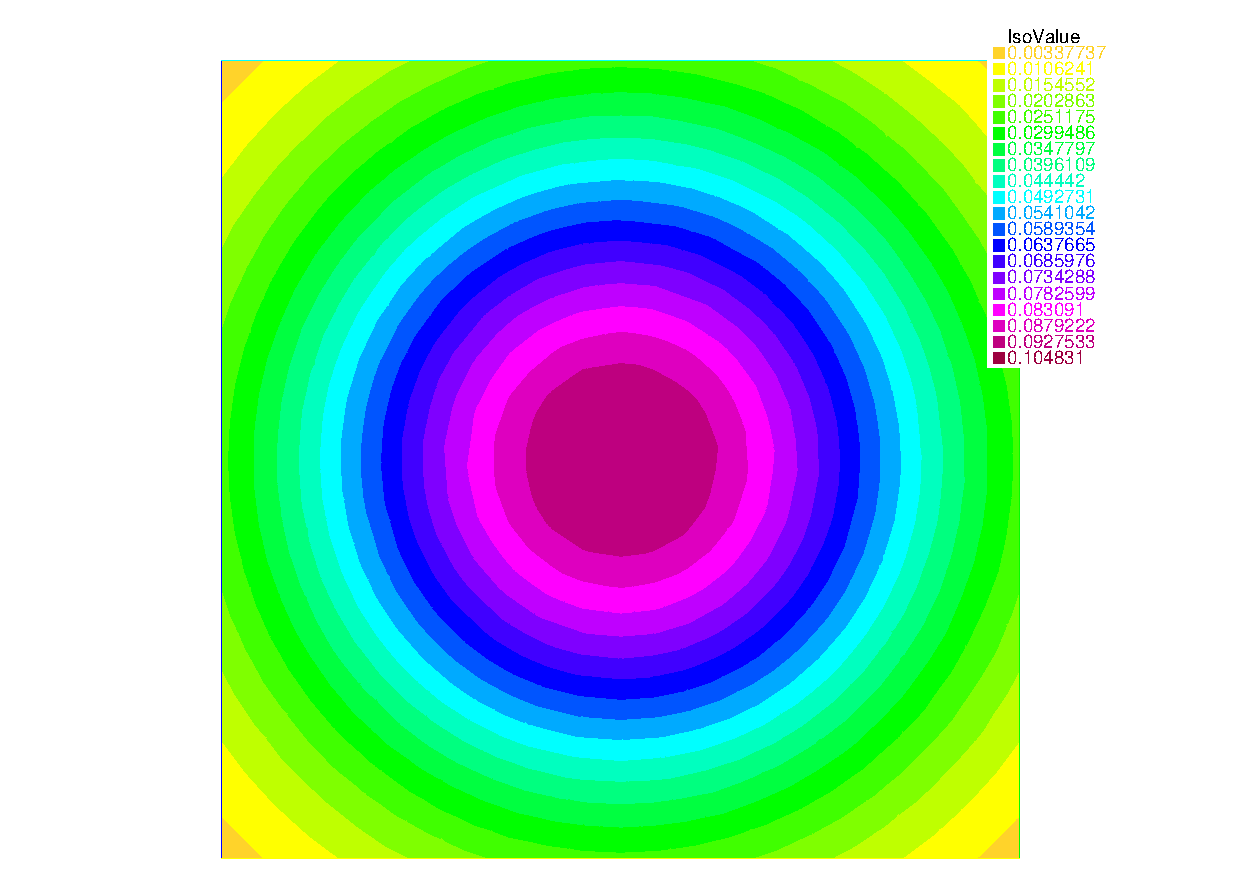
\includegraphics[width=0.55\textwidth]{additional/fem/initial.pdf}
			\caption{Распределение инфицированных в начальный момент времени}
		\end{figure}

	}

	\frame {

		\begin{multicols}{2}
			\begin{figure}[H]
				\centering
				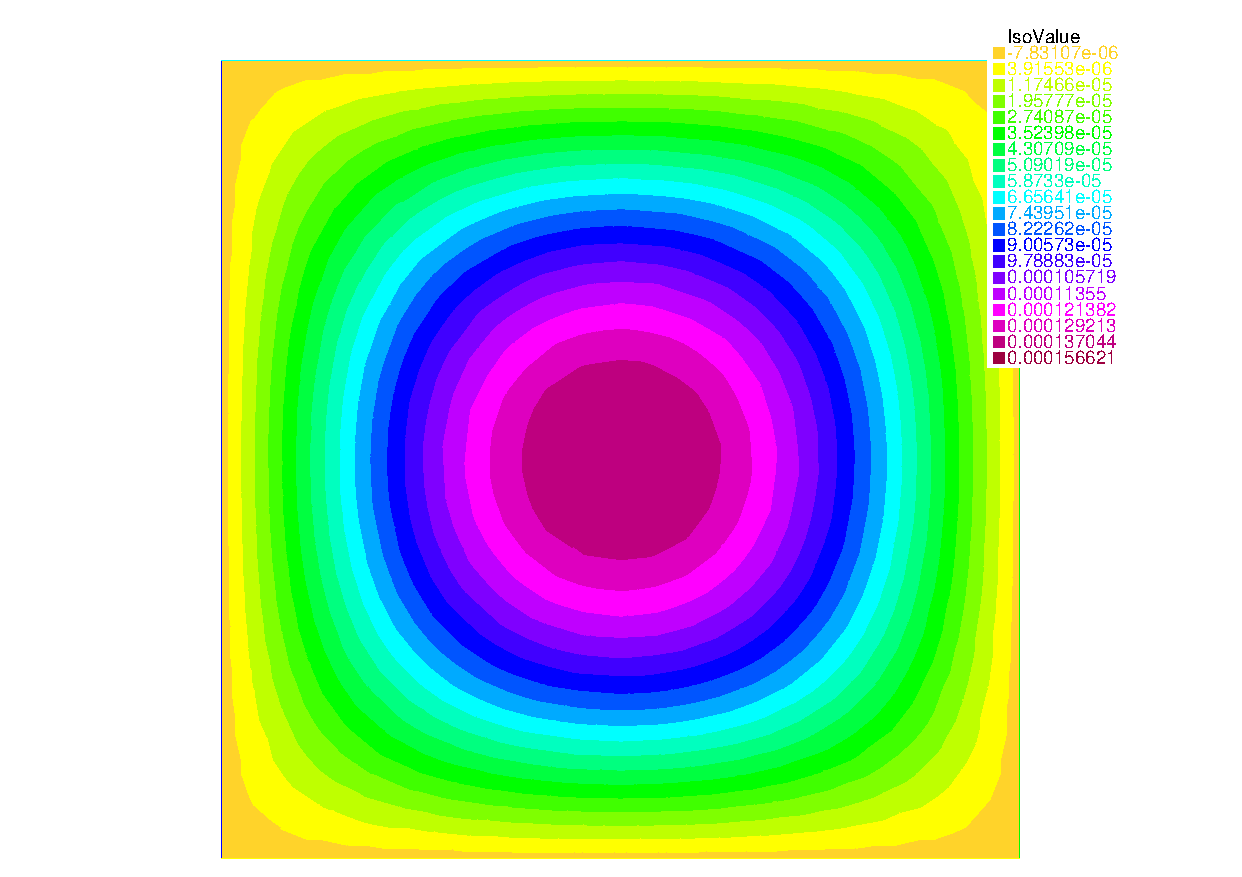
\includegraphics[width=0.6\textwidth]{additional/fem/middle.pdf}
				\caption{Распределение инфицированных момент, когда в область перестают поступать подверженные особи извне}
			\end{figure}

			\columnbreak

			\begin{figure}[H]
				\centering
				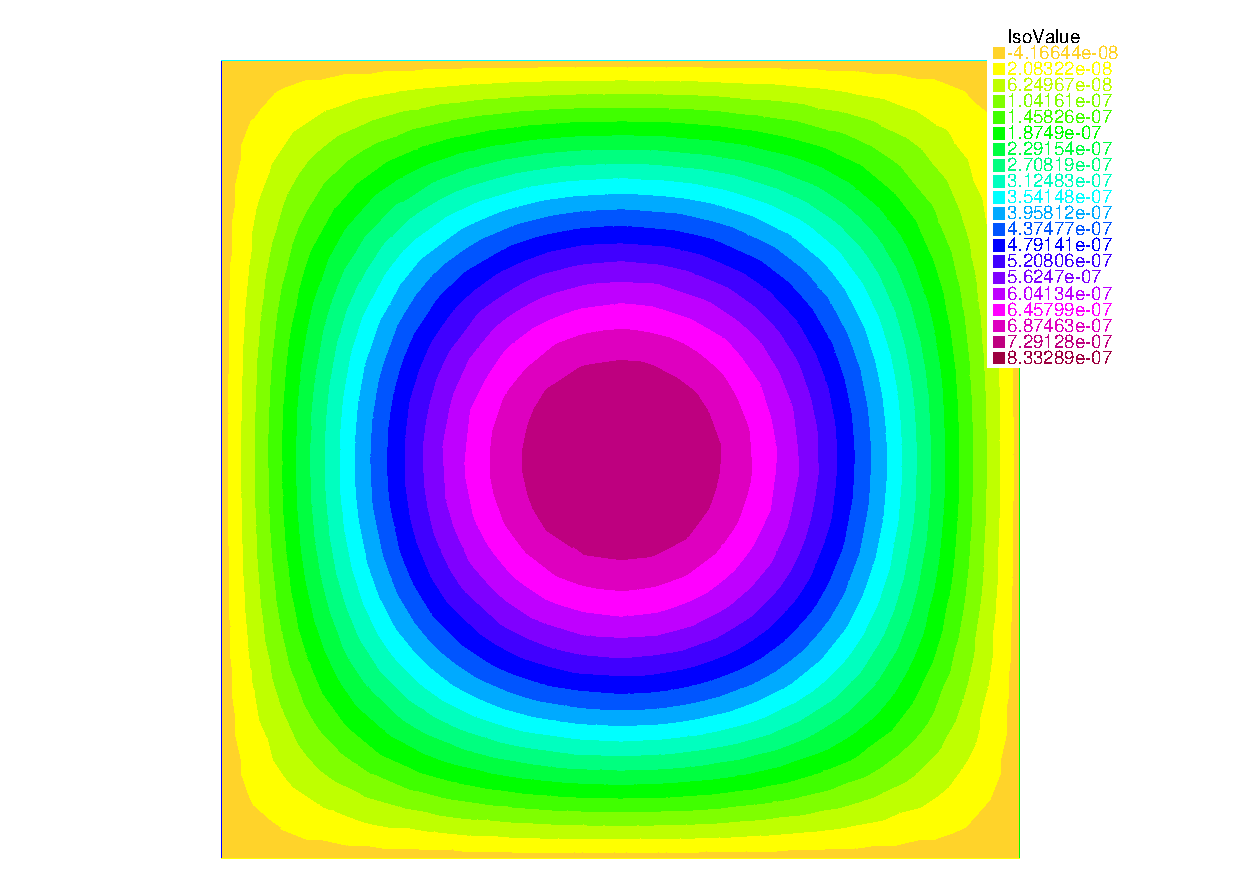
\includegraphics[width=0.6\textwidth]{../additional/fem/last.pdf}
				\caption{Распределение инфицированных в конечный момент времени}
			\end{figure}
		\end{multicols}
	}

	\frame {

		\frametitle{Публикации}

		\begin{thebibliography}{10}
    
			\bibitem{JVM21}
			Бризицкий Р.В., Максимов П.А. 
			Краевые и экстремальные задачи для нелинейного уравнения 
			реакции--диффузии--конвекции при условии Дирихле // ЖВМ. 2021

			\bibitem{CEUR}
			Brizitskii R.V., Chebotarev A.Yu., Bystrova V.S., Maksimov P.A.
			Theoretical and numerical analysis of extremum problems 
			for reaction-diffusion model //
			CEUR Workshop Proc. 2021. V. 2837. P. 77--87.

			\vspace{30pt}

			Подготовлена к отправке в Дифференциальные уравнения:

			\bibitem{Sib21}
			Бризицкий Р.В., Максимов П.А.
			Об устойчивости решений задач управления для нелинейного уравнения
			реакции-диффузии-конвекции

		\end{thebibliography}

	}


\end{document}